\part{Entrega 3}

\section{Introducción}

Este proyecto busca diseñar un datacenter orbital de 1MW para entrenar modelos de inteligencia artificial usando paneles solares en órbita. Esto se basara en la idea presentada por Lumen Orbit que busca realizar esto para datacenters de 40MW.

El objetivo de este informe es presentar dos diseños de estrcuturas para este datacenter, de forma de cumplir ciertas especificaciones de diseño y de operación. Donde los principales requerimientos son la capacidad de generar 1MW de energía, para lo cual se necesitaran de 3.334 $m^2$ de paneles solares. Además, se deben cumplir ciertas condiciones de diseño, como que la fracción de masa debe ser menor al 30\%, la frecuencia del primer modo debe ser mayor a 0.1Hz, la desangulación para un cambio de temperatura de 150\textdegree{}C debe ser menor a 2\textdegree{} y se debe cumplir con un factor de seguridad de 2.

Dentro de las especificaiones del satelite, este sera un rectangulo de 6.6 m x 2.6 m x 7.8 m y el material de la estructura de los paneles solares sera de fibra de carbono de alto modulo M55J. Dentro de las consideraciones el peso de al estrcutura y satelite no se consideranran como un priblema, solo que la estructura sea lo suficientemente rigida para soportar una aceleracion de 0.1g en cualquier direccion. 

Para llevar a cabo este estudio se utilizara el software de diseño de estructuras OpenSeesPy, el cual permite realizar análisis de elementos finitos de estructuras. Además, se utilizaran otros para la visualización de los resultados obtenidos. El objetivo de cada diseño es cumplir con los requerimientos de diseño y operación, y a la vez minimizar el peso total y el momento de inercia de todo este datacenter.

\newpage
\section{Condiciones de diseño y operación}

Para el desarrollo de esta estructura se buscan cumplir ciertas condiciones de diseño y operación, además, de asumir otras para simplificar el estudio del problema. 

Dentro de las condiciones de diseño estan:

\begin{itemize}
    \item Una potencia de 1 MW, considerando que los paneles solares tienen una eficiencia de 300 W/$m^2$.
    \item El peso de los paneles solares es de 1.1 kg/$m^2$.
    \item La fracción de masa debe ser menor al 30\%.
    \item La frecuencia del primer modo debe ser mayor a 0.1Hz.
    \item la estructura puede tener una aceleracion de 0.1g en cualquier direccion.
    \item La desangulación para un cambio de temperatura de 150\textdegree{}C debe ser menor a 2\textdegree.
    \item Se debe cumplir con un factor de seguridad de 2.
    \item Se utilizara el material compuesto de fibra de carbono de alto modulo M55J.
    \item El reticulado se puede apoyar de cualquier forma en el satelite.
    \item El satelite sera un rectangulo de 6.6 m x 2.6 m x 7.8 m.
\end{itemize}

Luego a medida que se fue realizando el diseño se fueron asumiendo ciertas condiciones apartes de las ya nombradas, estas son:

\begin{itemize}
    \item El peso de la estructura y satelite no se consideran como un problema, pero si se busca minimizarlo.
    \item Se utilizaran distintas barras para la estructura, las cuales se deciden para optimizar la masa de la estructura.
    \item Los nodos del 1 al 8 son los nodos que conforman el satelite y estan fijos en el espacio.
\end{itemize}

\newpage
\section{Propuesta 1}

En esta propuesta se considero que la estructura seria un reticulado de barras donde saldrian 4 "brazos" del satelite, donde se utilizan barras de distintos tamaños para optimizar la masa de la estructura. Este diseño se decidio ya que al ser 4 brazos independientes uno del otro seria facil de manipular en el sofware en el que se estudia la estructura. Además, cabe mencionar que este diseño se baso, aunque no es del todo igual, del diseño de SpideWeb del (citar trussselator), donde se puede ver que este diseño tiene 8 brazos, aunque en base a la prueba y error la llevamos a solo 4 brazos, asi minimizar la masa de estructura manteniendo todos los criterios necesarios. Quedando de la siguinte forma: 

\begin{figure}[H]
    \centering
    \includegraphics[width=0.8\textwidth]{GRAFICOS_DISENO_LUKAS/diseño_satelite.png}
    \caption{Diseño de la propuesta 1 para el satelite}
    \label{fig:propuesta1}
\end{figure}

Como se dijo anteriormente, se puede apreciar los 4 "brazos" que salen del satelite, donde se puede ver que cada uno de estos tiene la misma distancia y la existencia de 5 tipos de barras, esto criterio lo realizo pyhton de forma de optimizar la masa de la estrcutura y cumplir con los requerimientos de diseño.

\subsection{Análisis de la estructura}

A continuacion se mostraran los resultados de los criterios exigidos para el diseño de la estructura.

\begin{figure}[H]
    \centering
    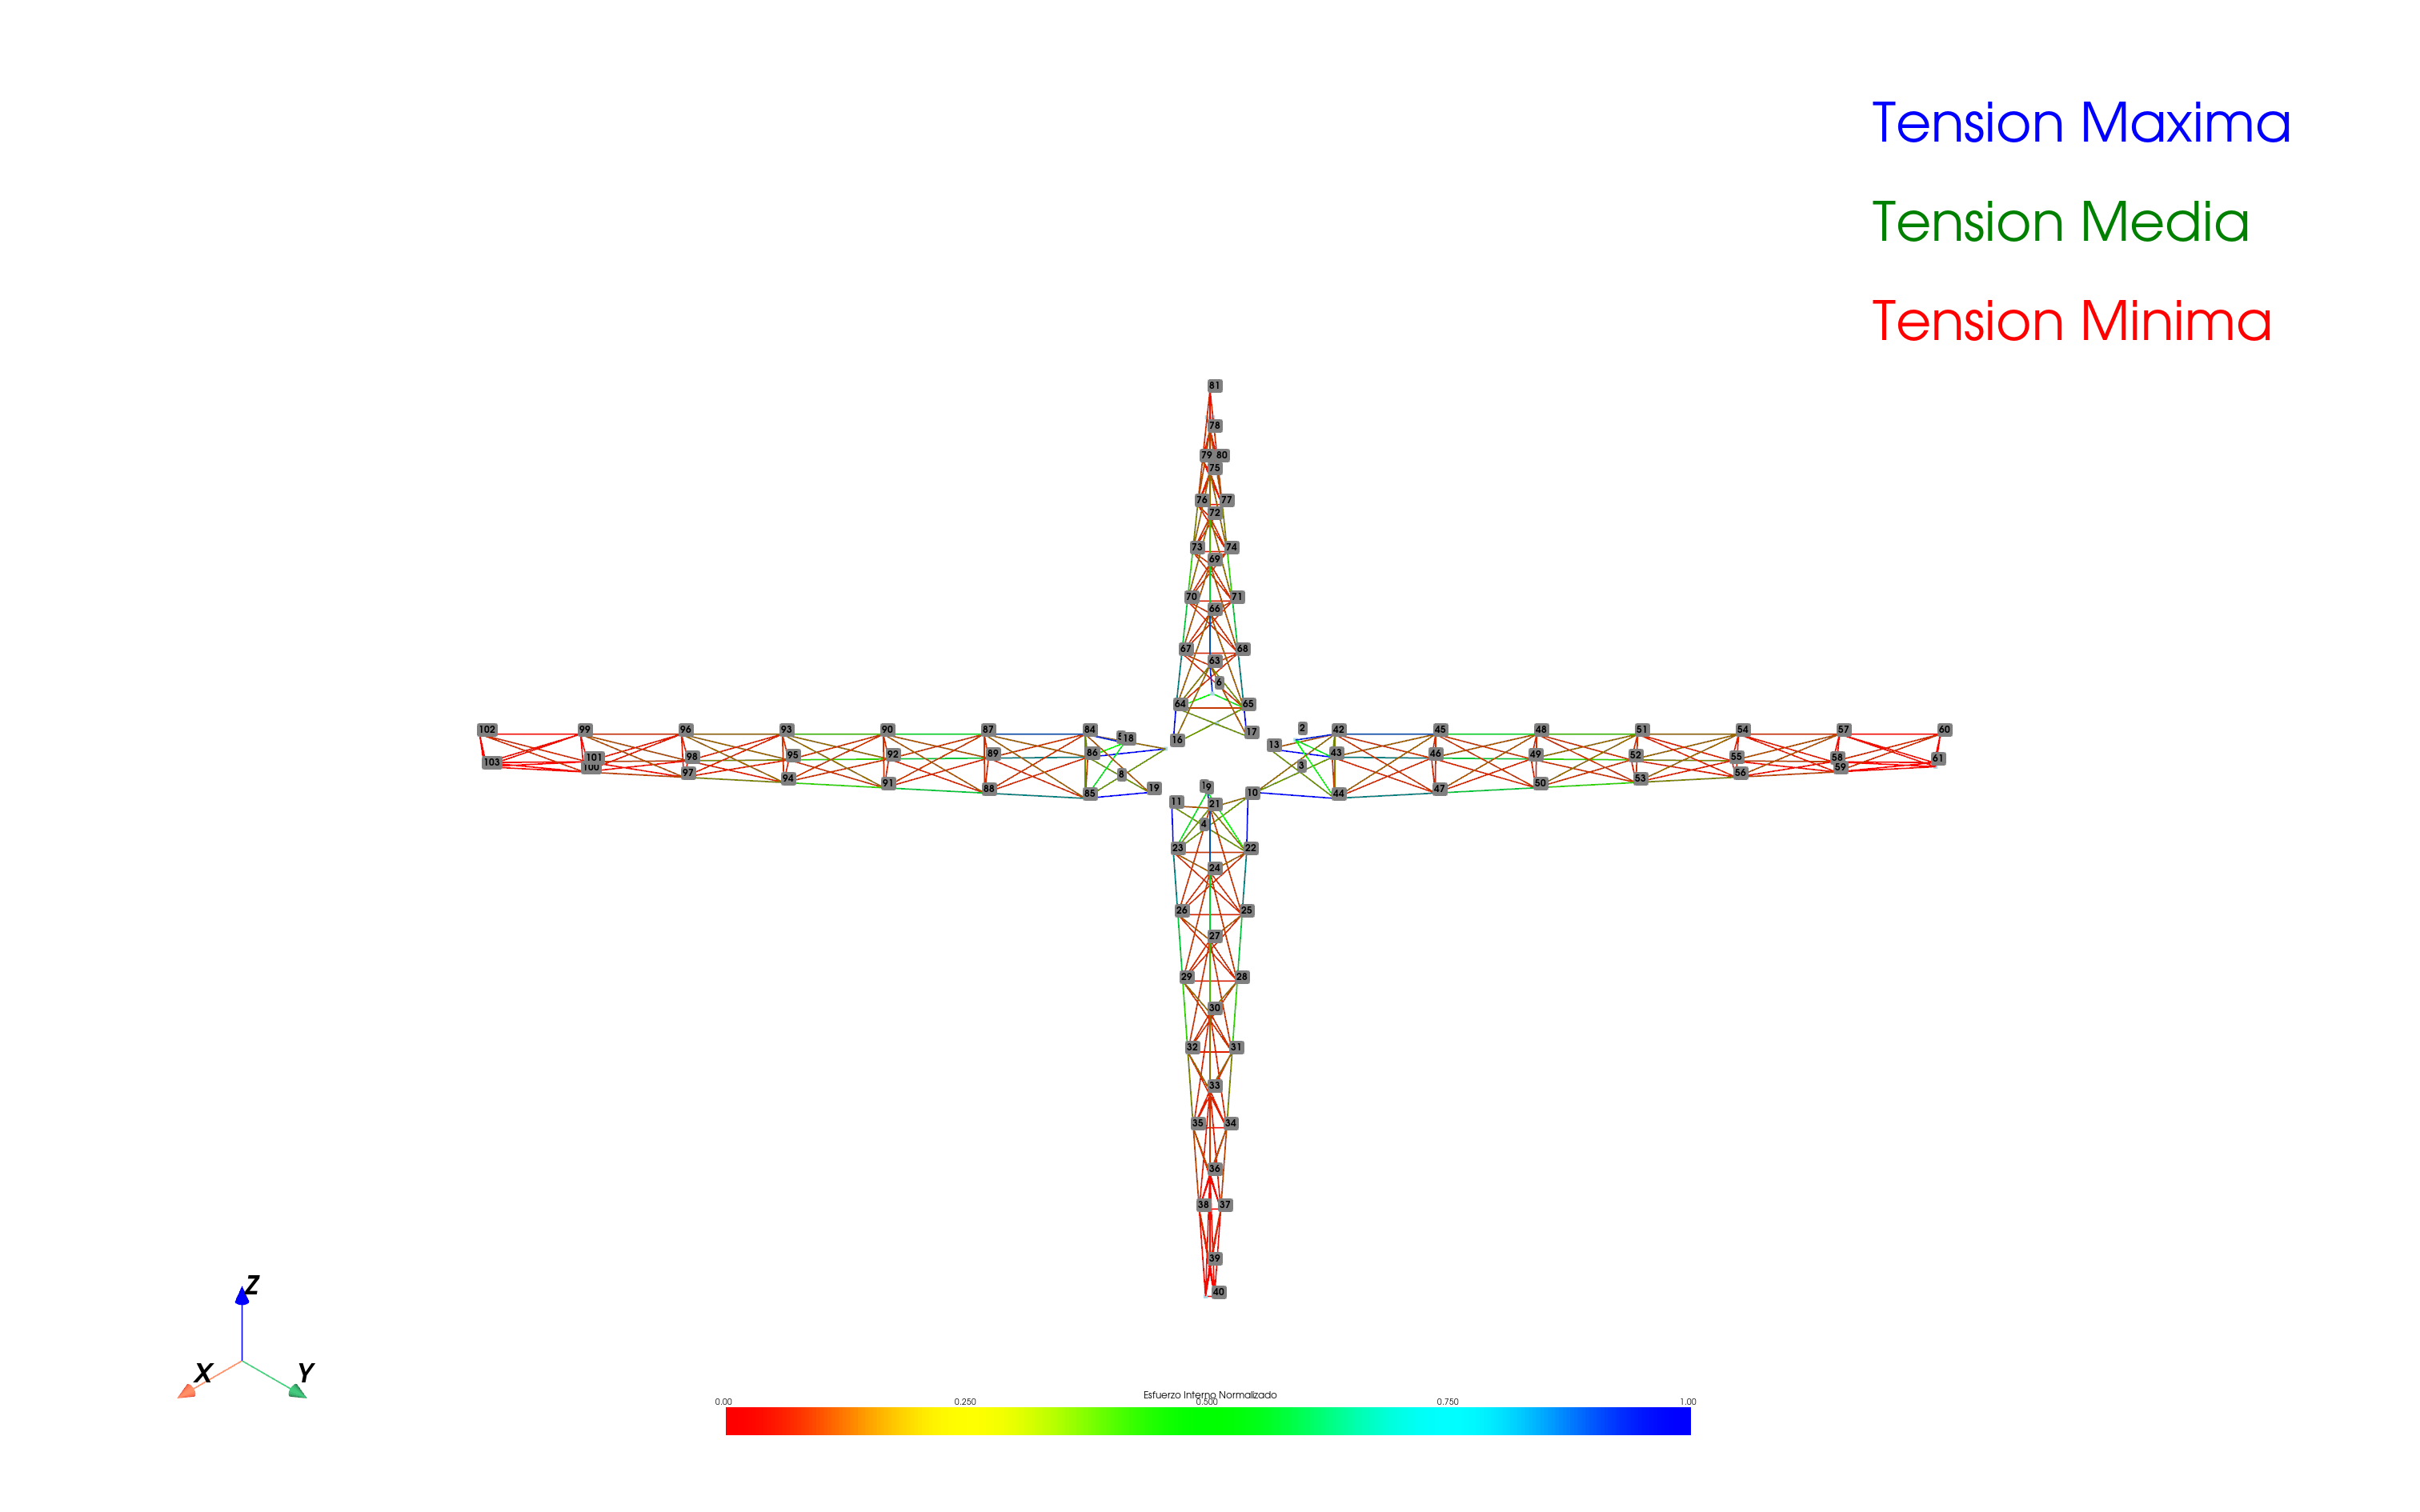
\includegraphics[width=0.8\textwidth]{GRAFICOS_DISENO_LUKAS/esfuerzo_barras_inercia.png}
    \caption{Esfuerzo interno de las barras}
    \label{fig:propuesta1_ei}
\end{figure}

En la figura \ref{fig:propuesta1_ei} se puede ver que el esfuerzo interno de las barras disminuye a medida que uno se aleja del satelite. Esto se debe a que las barras mas cercanas al satelite son las que soportan la mayor parte de la carga, por lo que se ven mas afectadas por esta.

\begin{figure}[H]
    \centering
    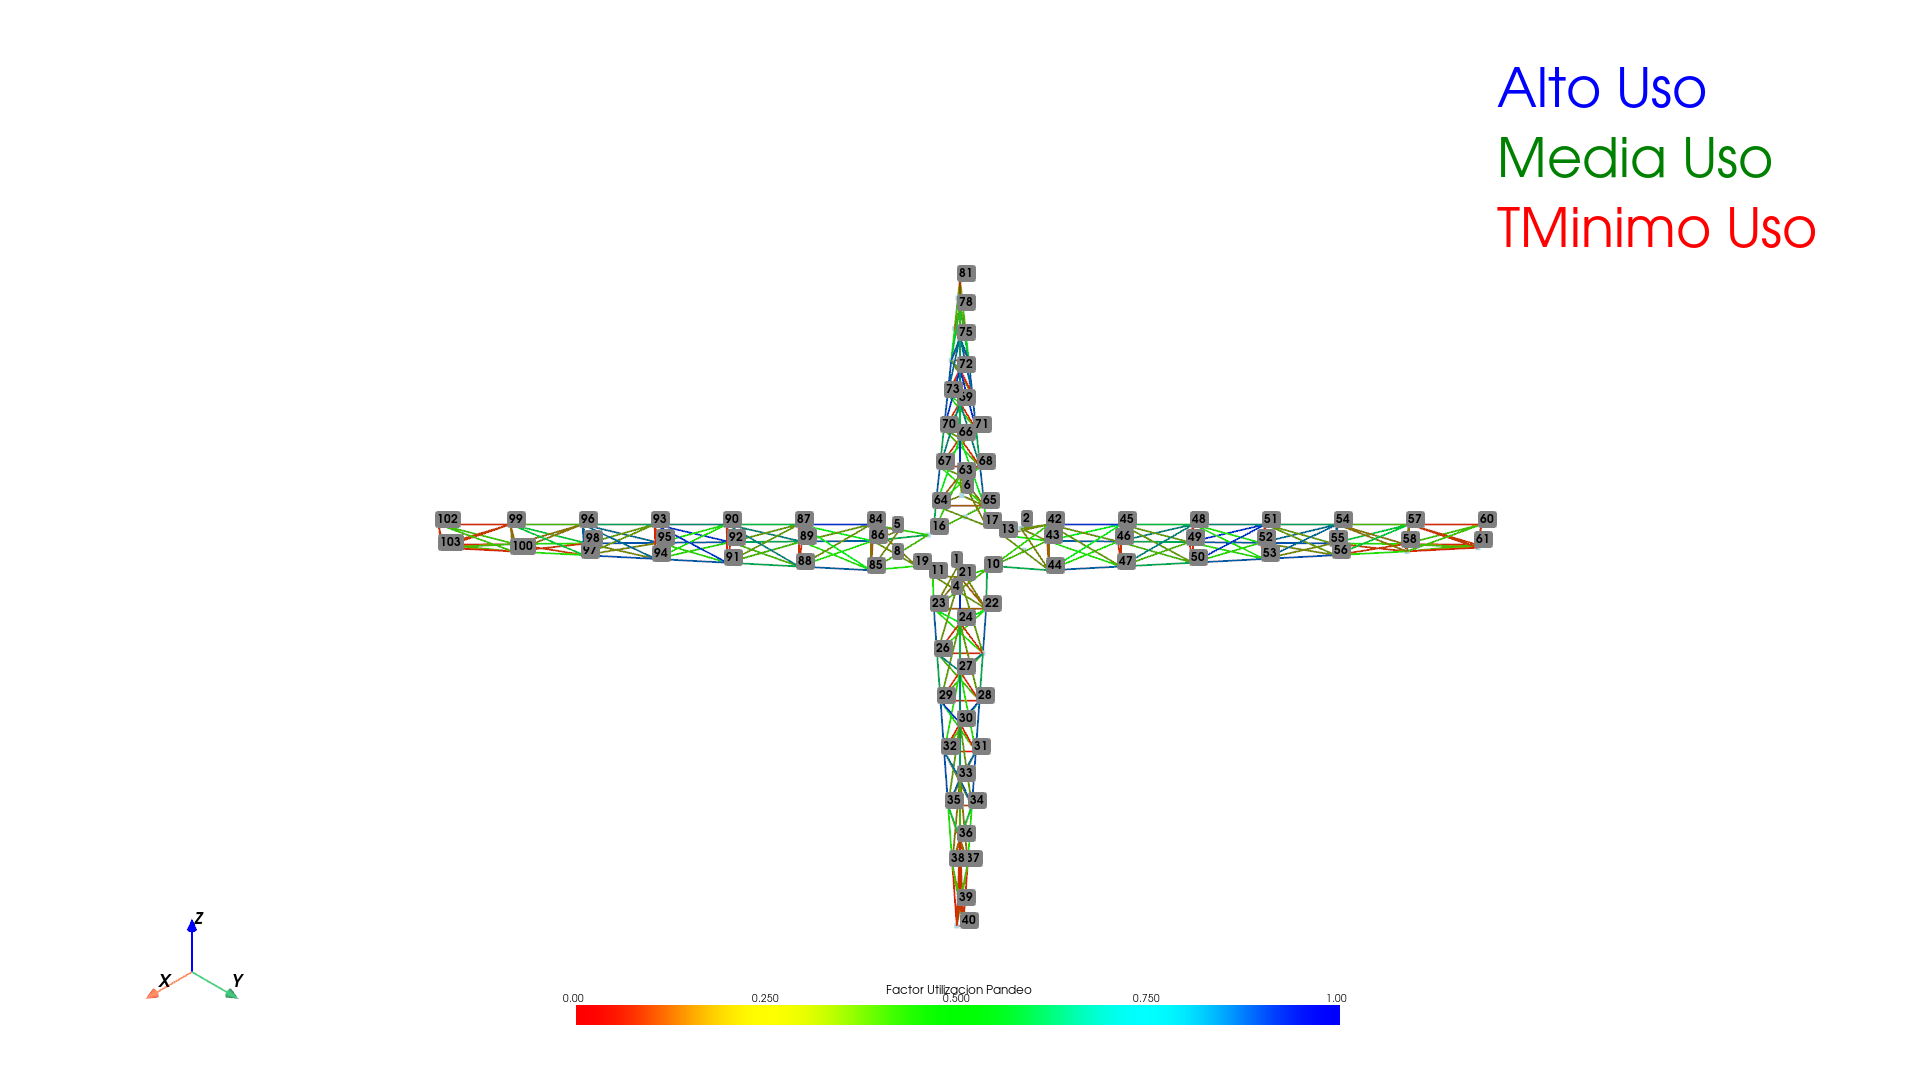
\includegraphics[width=0.8\textwidth]{GRAFICOS_DISENO_LUKAS/factor_utilizacion_pandeo.png}
    \caption{Pandeo de la estrcutura}
    \label{fig:propuesta1_pandeo}
\end{figure}

En la figura \ref{fig:propuesta1_pandeo}, esto es un factor a tener en cuenta, ya que, las barras es mas probable que fallen por pandeo, es por eso que lass barras se decidieron para que cumplieran todo los criterios y con un factor de seguridad de 2.

\begin{figure}[H]
    \centering
    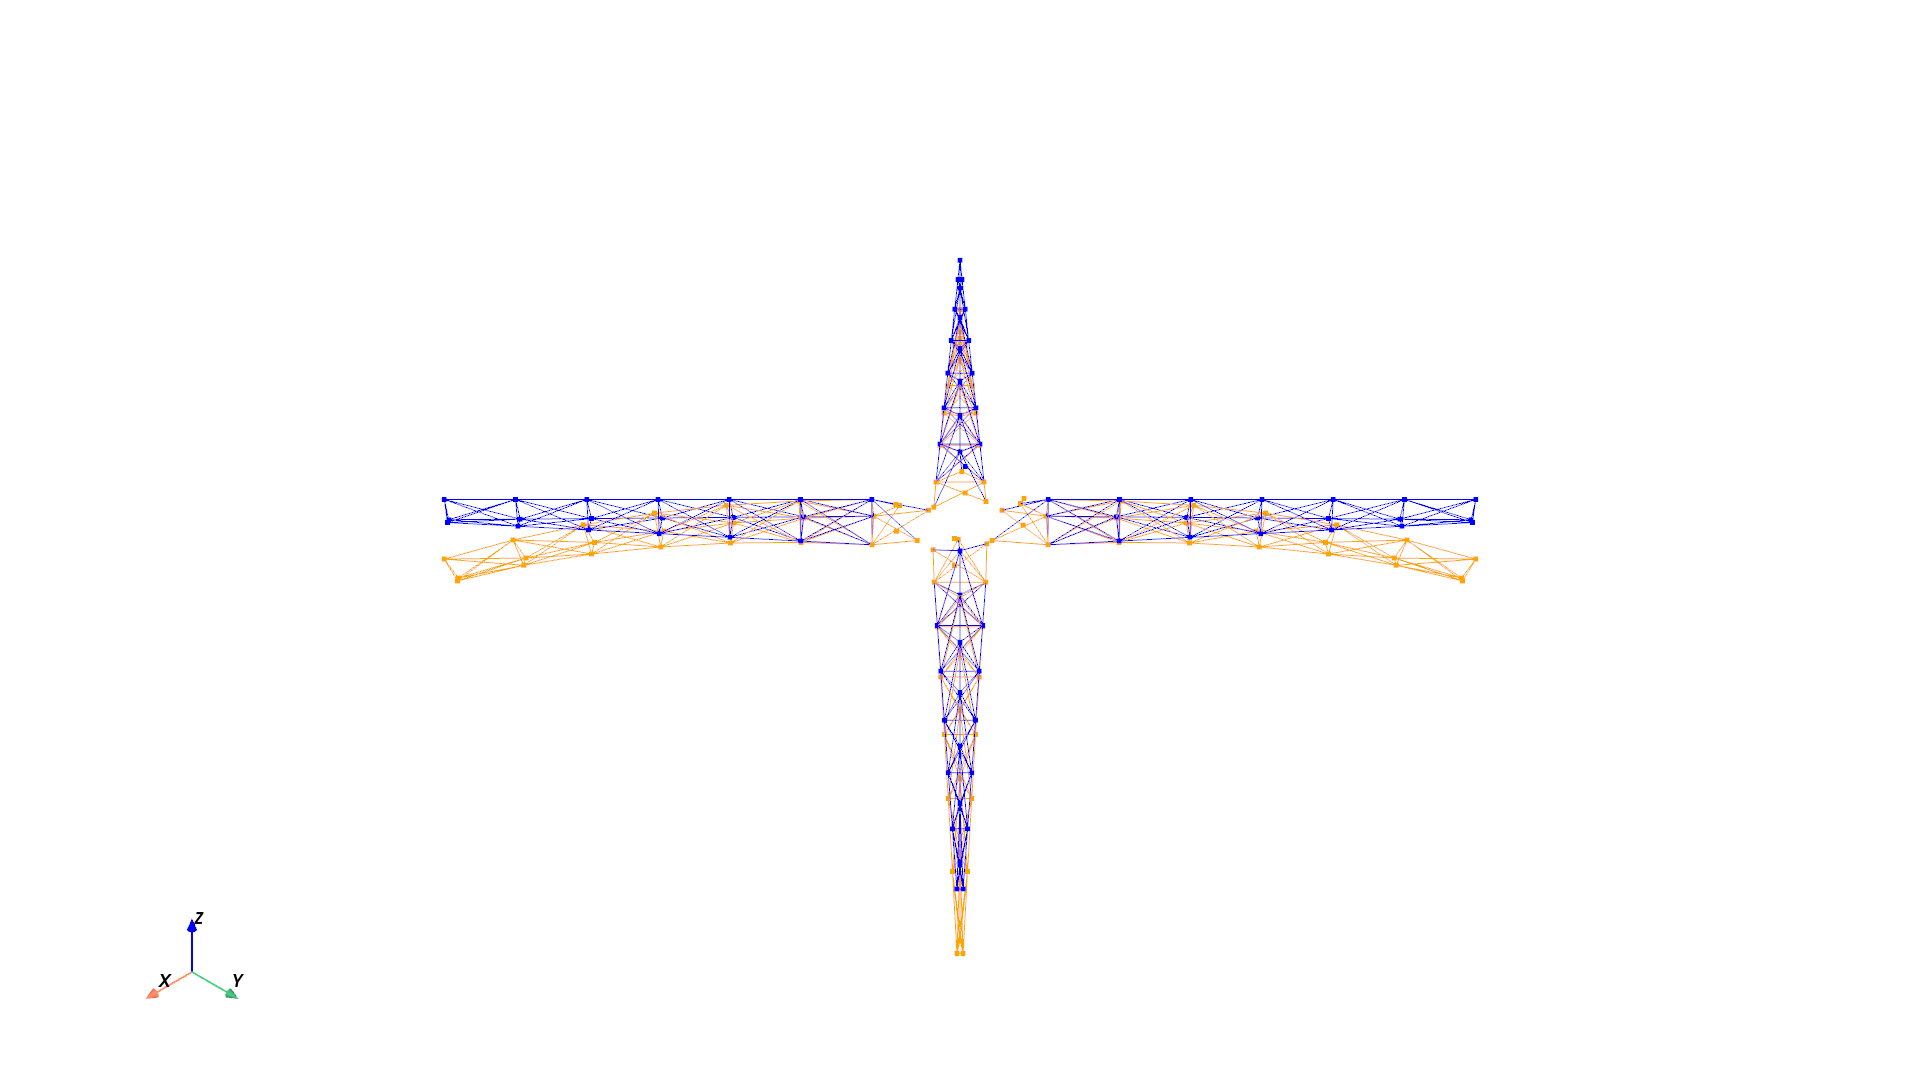
\includegraphics[width=0.8\textwidth]{GRAFICOS_DISENO_LUKAS/desplazamiento_termico.png}
    \caption{Desplazamiento termico de la estrcutura}
    \label{fig:propuesta1_termico}
\end{figure}

En la figura \ref{fig:propuesta1_termico} se puede apreciar el desplazamiento termico, donde se asumio que solamente las barras que estan junta al panel solar son las que se ven afectadas por el cambio de temperatura, esto ya que reciben el calor directamente.

\newpage
\section{Propuesta 2}

En este caso el diseño tine una forma de H, donde se decidio llevar a cabo este diseño, ya que se considero que podia ser un buen punto medio entre la masa de la estructura y su rigidez. Este diseño tambien se baso en el diseño presentado en (Citar trussselator). quedando de la siguiente forma:

\begin{figure}[H]
    \centering
    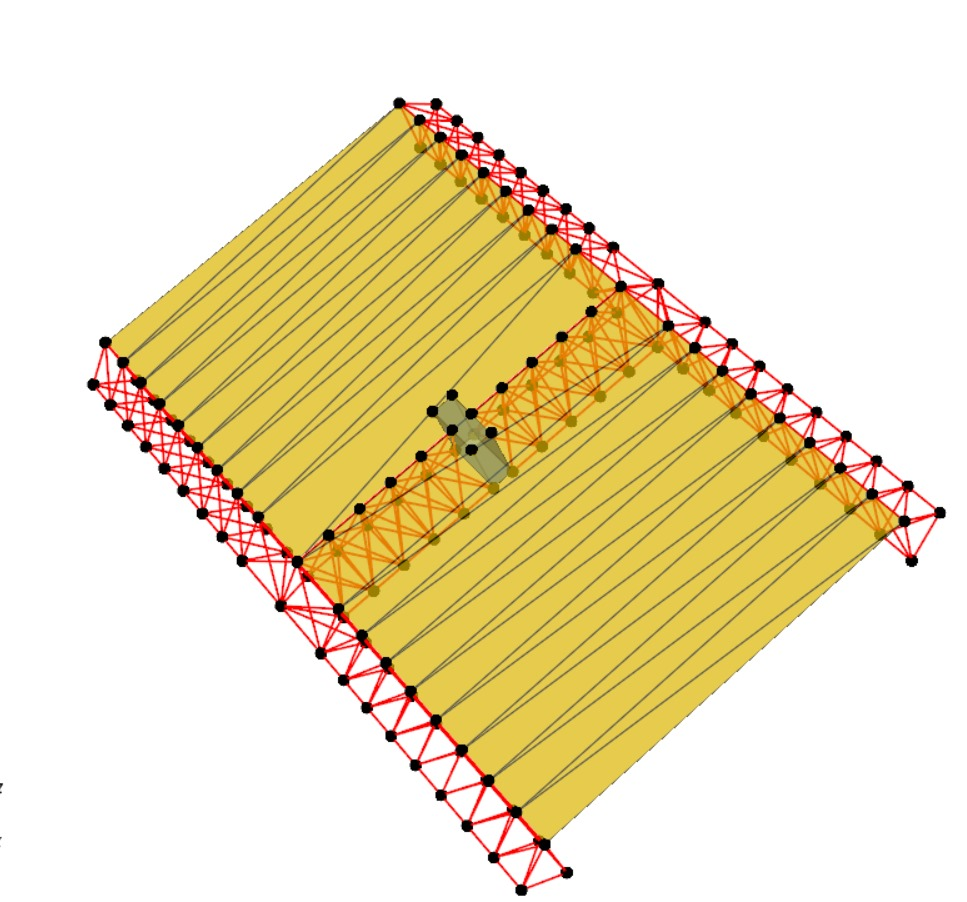
\includegraphics[width=0.8\textwidth]{GRAFICOS_DISENO_BENO/propuesta2.png}
    \caption{Diseño de la propuesta 2 para el satelite}
    \label{fig:propuesta2}
\end{figure}

\newpage
\section{Comparación de propuestas}


\newpage
\section{Propuesta final}

Luego de comparar amabas propuestas, se decidio que la propuesta 1 es la que cumple con todos los criterios de diseño y operación, por lo que se decidio que esta es la mejor propuesta para el diseño del datacenter orbital de 1MW. Además, esta propuesta es la que minimiza el peso total y el momento de inercia de todo el datacenter. Luego otro criterio utilizado para elegir este diseño es que al ser 4 brazos independientes unos de otros, al tener cualquier complicacion es mas facil de trabajar en el software de diseño de estructuras OpenSeesPy por lo que se seguira con este diseño para el resto del proyecto.

\begin{figure}[H]
    \centering
    \includegraphics[width=0.8\textwidth]{GRAFICOS_DISENO_LUKAS/diseño_satelite.png}
    \caption{Diseño final (Propuesta 1)}
    \label{fig:propuesta1}
\end{figure}

